% Copyright 2004 by Till Tantau <tantau@users.sourceforge.net>.
%
% In principle, this file can be redistributed and/or modified under
% the terms of the GNU Public License, version 2.
%
% However, this file is supposed to be a template to be modified
% for your own needs. For this reason, if you use this file as a
% template and not specifically distribute it as part of a another
% package/program, I grant the extra permission to freely copy and
% modify this file as you see fit and even to delete this copyright
% notice. 

\documentclass{beamer}
% Replace the \documentclass declaration above
% with the following two lines to typeset your 
% lecture notes as a handout:
%\documentclass{article}
%\usepackage{beamerarticle}

\usepackage{graphicx}
\usepackage[utf8]{inputenc}
 
\graphicspath{ {img/} }


% There are many different themes available for Beamer. A comprehensive
% list with examples is given here:
% http://deic.uab.es/~iblanes/beamer_gallery/index_by_theme.html
% You can uncomment the themes below if you would like to use a different
% one:
%\usetheme{AnnArbor}
%\usetheme{Antibes}
%\usetheme{Bergen}
%\usetheme{Berkeley}
%\usetheme{Berlin}
%\usetheme{Boadilla}
%\usetheme{boxes}
%\usetheme{CambridgeUS}
%\usetheme{Copenhagen}
%\usetheme{Darmstadt}
%\usetheme{default}
%\usetheme{Frankfurt}
%\usetheme{Goettingen}
%\usetheme{Hannover}
%\usetheme{Ilmenau}
%\usetheme{JuanLesPins}
%\usetheme{Luebeck}
%\usetheme{Madrid}
%\usetheme{Malmoe}
%\usetheme{Marburg}
%\usetheme{Montpellier}
%\usetheme{PaloAlto}
%\usetheme{Pittsburgh}
%\usetheme{Rochester}
%\usetheme{Singapore}
%\usetheme{Szeged}
\usetheme{Warsaw}

\title{Programming with NodeJS}

% A subtitle is optional and this may be deleted
\subtitle{Lesson 2: Callbacks, buffers, streams, APIs and Express}

%\author{F.~Author\inst{1} \and S.~Another\inst{2}}
% - Give the names in the same order as the appear in the paper.
% - Use the \inst{?} command only if the authors have different
%   affiliation.

%\institute[Universities of Somewhere and Elsewhere] % (optional, but mostly needed)
%{
%  \inst{1}%
%  Department of Computer Science\\
%  University of Somewhere
%  \and
%  \inst{2}%
%  Department of Theoretical Philosophy\\
%  University of Elsewhere}
% - Use the \inst command only if there are several affiliations.
% - Keep it simple, no one is interested in your street address.

\date{Febuary 14th, 2017}
% - Either use conference name or its abbreviation.
% - Not really informative to the audience, more for people (including
%   yourself) who are reading the slides online

\subject{NodeJS Lessons}
% This is only inserted into the PDF information catalog. Can be left
% out. 

% If you have a file called "university-logo-filename.xxx", where xxx
% is a graphic format that can be processed by latex or pdflatex,
% resp., then you can add a logo as follows:

% \pgfdeclareimage[height=0.5cm]{university-logo}{university-logo-filename}
% \logo{\pgfuseimage{university-logo}}

% Delete this, if you do not want the table of contents to pop up at
% the beginning of each subsection:
%\AtBeginSubsection[]
%{
%  \begin{frame}<beamer>{Outline}
%    \tableofcontents[currentsection,currentsubsection]
%  \end{frame}
%}

% Let's get started
\begin{document}

\begin{frame}
  \titlepage
\end{frame}

%\begin{frame}{Outline}
%  \tableofcontents
%  % You might wish to add the option [pausesections]
%\end{frame}

% Section and subsections will appear in the presentation overview
% and table of contents.
\section{Introduction}

\begin{frame}{Summary of last week}
  Last week we:
  \pause
  \begin{itemize}
  \item We have installed NodeJS and NPM\pause
  \item We have learnt about JS syntax\pause
  \item We have learnt about NodeJS and what it's useful for\pause
  \item We have made a very simple http server
  \end{itemize}
\end{frame}

\section{Callbacks and the Event Loop}

\begin{frame}{Callbacks? Huh?}

NodeJS is a language developed around the idea of everything being asynchronous. \\
\pause
Asynchronous programming is programming where an operation is executed after the previous one has been terminated.\\
\pause
How does asynchronous programming differ from normal programming?\\ 
\pause
Consider this example:


\end{frame}

\begin{frame}{Asynchronous programming example}
Say you really want to have a chat with your mate Paul about the weather. You have two ways to get in touch with him.
You can either: \pause
\begin{itemize}
  \item Phone him\pause
  \item Send him a letter
\end{itemize}

\end{frame}

\begin{frame}

Both have distinct advantages and disadvantages.\\
\pause
If you phone him and ask him what the weather is like, you have to sit there and wait for him to look outside and reply.\\
\pause
This is considered synchronous. You have a guarantee that he will reply as soon as possible, but you have to wait the entire time he's looking outside.\\
\pause
Alternatively, if you send him a letter asking what the weather is like, you can do other things while you wait for the postman to come with his response. However, you have no idea how long until you will recieve that response is.\\
\pause
This is considered asynchronous.

\end{frame}

\begin{frame}

NodeJS is asynchronous.\\ \pause
The reason for this is just the same as with Paul and the weather. \pause If instead of talking to just Paul, you want to talk to 100s of people about the weather they are all experiencing, an asynchronous approach will allow you to keep conversations open with all of these people at the same time.\\

\end{frame}

\begin{frame}{Seperating IO bound and CPU bound tasks}

Note, this asynchronous feature is really strong for some purposes and really weak for others.\\
There are two types of functionality we will want in our program. They are:
\pause
\begin{itemize}
  \item CPU bound \pause - stuff which the CPU has to do e.g. sorting an array, adding numbers together \pause
  \item I/O bound \pause - stuff which the CPU tells something else to do, where it then gives it back to the CPU at another time e.g. opening a file (your hard drive takes time to retrieve the file), downloading something from the web (your network card takes time to download)
\end{itemize}

\pause

This distinction is important for NodeJS as it defines which bits NodeJS can do seemingly concurrently and which it won't be able to do well.

\end{frame}

\begin{frame}{NodeJS and concurrency}

Specifically, NodeJS is a single threaded program which uses an event loop to manage pseudo-concurrency. \\
\pause
What this means is that, if NodeJS is doing a CPU bound task, the entire program has to stop and wait for the CPU task to be completed before \textbf{anything} can happen.\\
\pause
If however NodeJS is executing an IO bound task, it can say "ok you do that IO, and once you've done the IO task, tell me and i'll execute this bit of code".\\
\pause
The "bit of code" is called a callback function and is a function which you give to an IO bound function, which is executed once the IO bound function is done.

\end{frame}

\begin{frame}{Callbacks}

\begin{figure}[h]
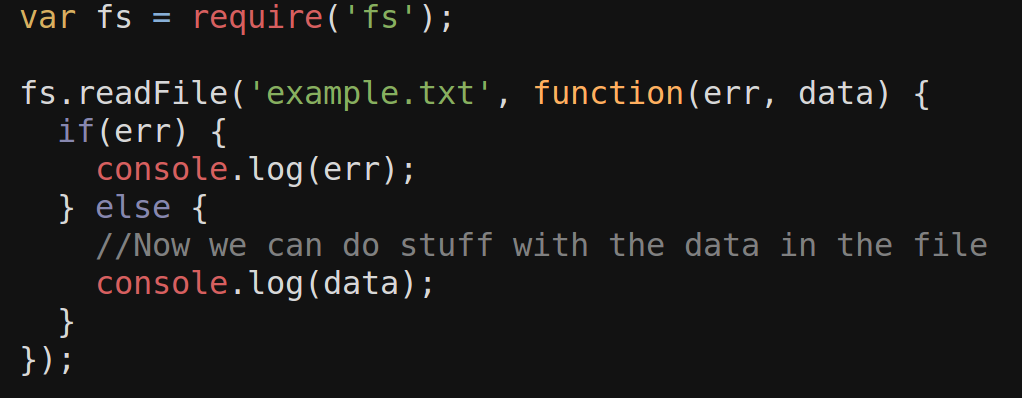
\includegraphics[width=0.8\textwidth]{fscode}
\end{figure}

\end{frame}

\begin{frame}{Callbacks}

\begin{figure}[h]
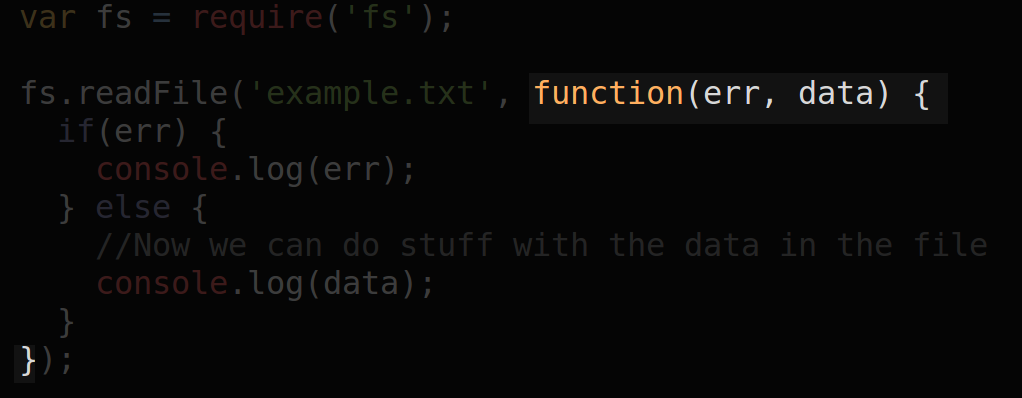
\includegraphics[width=0.8\textwidth]{fscode2}
\end{figure}

\end{frame}

\begin{frame}{Buffers}

Buffers are a class in NodeJS which allows us to deal with big chunks of bytes.\\
\pause
Useful for times where you're getting a chunk of bytes in from somewhere e.g. downloading a file or opening a file from your file system

\end{frame}

\begin{frame}{Buffers}

You can make a new buffer with \textit{var myBuffer = new Buffer(BUFFER SIZE);}.\\
\pause
You can write to a buffer via \textit{myBuffer.write(CONTENT);}.\\
\pause
Most usefully, you can convert a buffer to a string with \textit{myBuffer.toString()}.

\end{frame}

\begin{frame}{The Express framework}

The Express framework is an HTTP server framework for NodeJS with a bunch of really powerful features, making it much stronger than the framework we used last week, 'http'.


\end{frame}

\begin{frame}{Hello world in Express}

\begin{figure}[h]
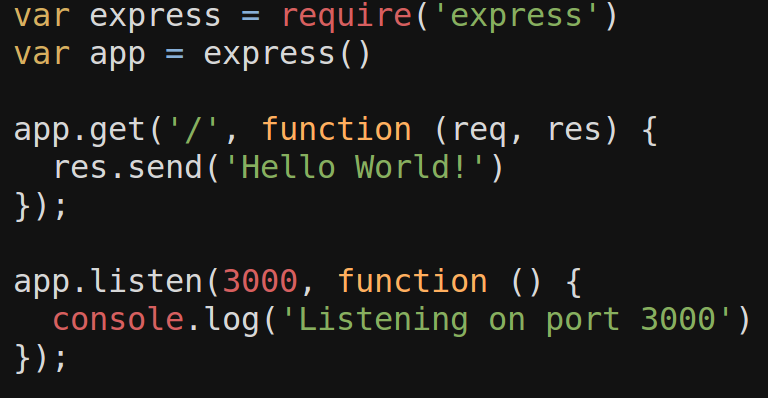
\includegraphics[width=0.8\textwidth]{express}
\end{figure}


\end{frame}

\begin{frame}{Hello world in Express}

\begin{figure}[h]
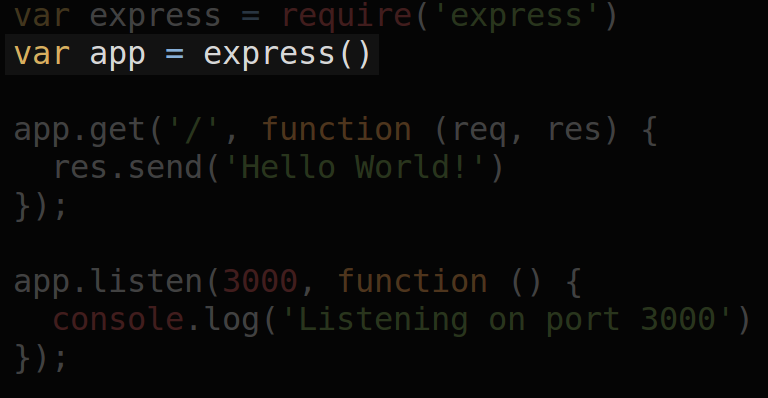
\includegraphics[width=0.8\textwidth]{express2}
\end{figure}


\end{frame}

\begin{frame}{Hello world in Express}

\begin{figure}[h]
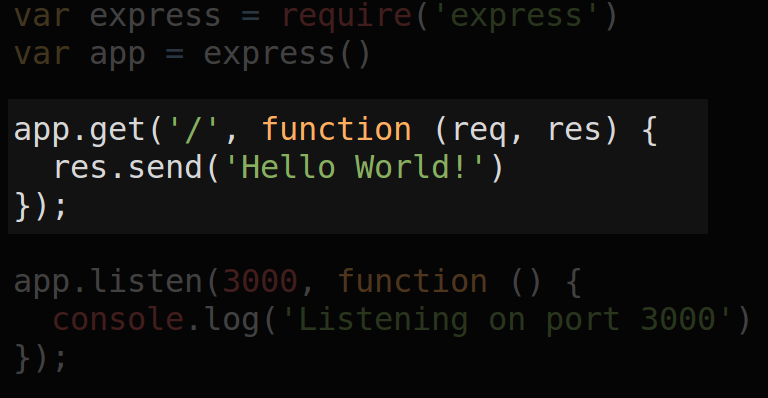
\includegraphics[width=0.8\textwidth]{express3}
\end{figure}


\end{frame}

\begin{frame}{Hello world in Express}

\begin{figure}[h]
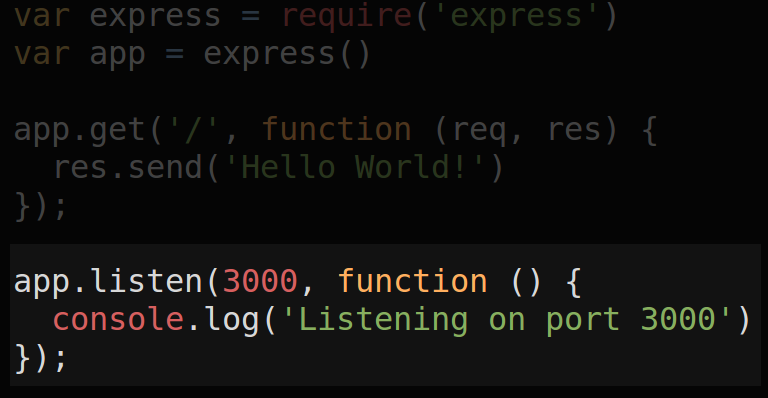
\includegraphics[width=0.8\textwidth]{express4}
\end{figure}


\end{frame}

\begin{frame}{Middleware}

One of the strong points of Express is it's middleware capabilities.\pause Middleware is code which is executed inbetween when you get the request and when you deal with it.\pause Some examples of middleware include adding authentication to every request, so only people who are logged in can go to certain places in the site.

\end{frame}

\begin{frame}{Endpoints}

An endpoint is a \textit{destination}. When you go to 127.0.0.1:3000 you are going to the root endpoint \textit{/}.\pause \\
If instead you go to 127.0.0.1:3000/hello/world, you are going to the endpoint \textit{/hello/world}.

\end{frame}

\begin{frame}{Templates}

Templates are pretty much HTML++.\\ \pause
They are pre-rendered on the server side and can be passed in values.

\end{frame}

\begin{frame}{EJS}

EJS is a templating language developed to be very strong when paired with javascript (like NodeJS). It mixes normal HTML with embedded javascript which is compiled before it is sent to the client. It looks a little like this:

\begin{figure}[h]
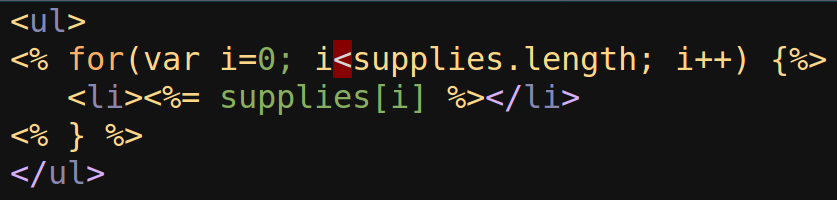
\includegraphics[width=0.6\textwidth]{ejs}
\end{figure}


\end{frame}

\begin{frame}{Putting it all together}

\end{frame}

\section{Summary}

\begin{frame}{That's all for tonight!}
  To summarise:
  \begin{itemize}
  \item We have learnt about callbacks and the NodeJS event loop
  \item We have learnt about buffers
  \item We have learnt about the Express framework
  \item We have made a complex server using Express
  \end{itemize}
\end{frame}

\begin{frame}{For next week}
Source code plus lecture slides will be available online soon after the lesson.\\
If you are new to HackSocNotts, please join us on \textit{http://hacksocnotts.slack.com}.\\
If you have any questions, feel free to ask now or over slack.\\
\end{frame}

\end{document}


